\section{Problem 2D: Larger stochastic SEIIaR Commuter model}

\subsection{a) 10 city simulation}

\begin{figure}[htb]
	\centering
	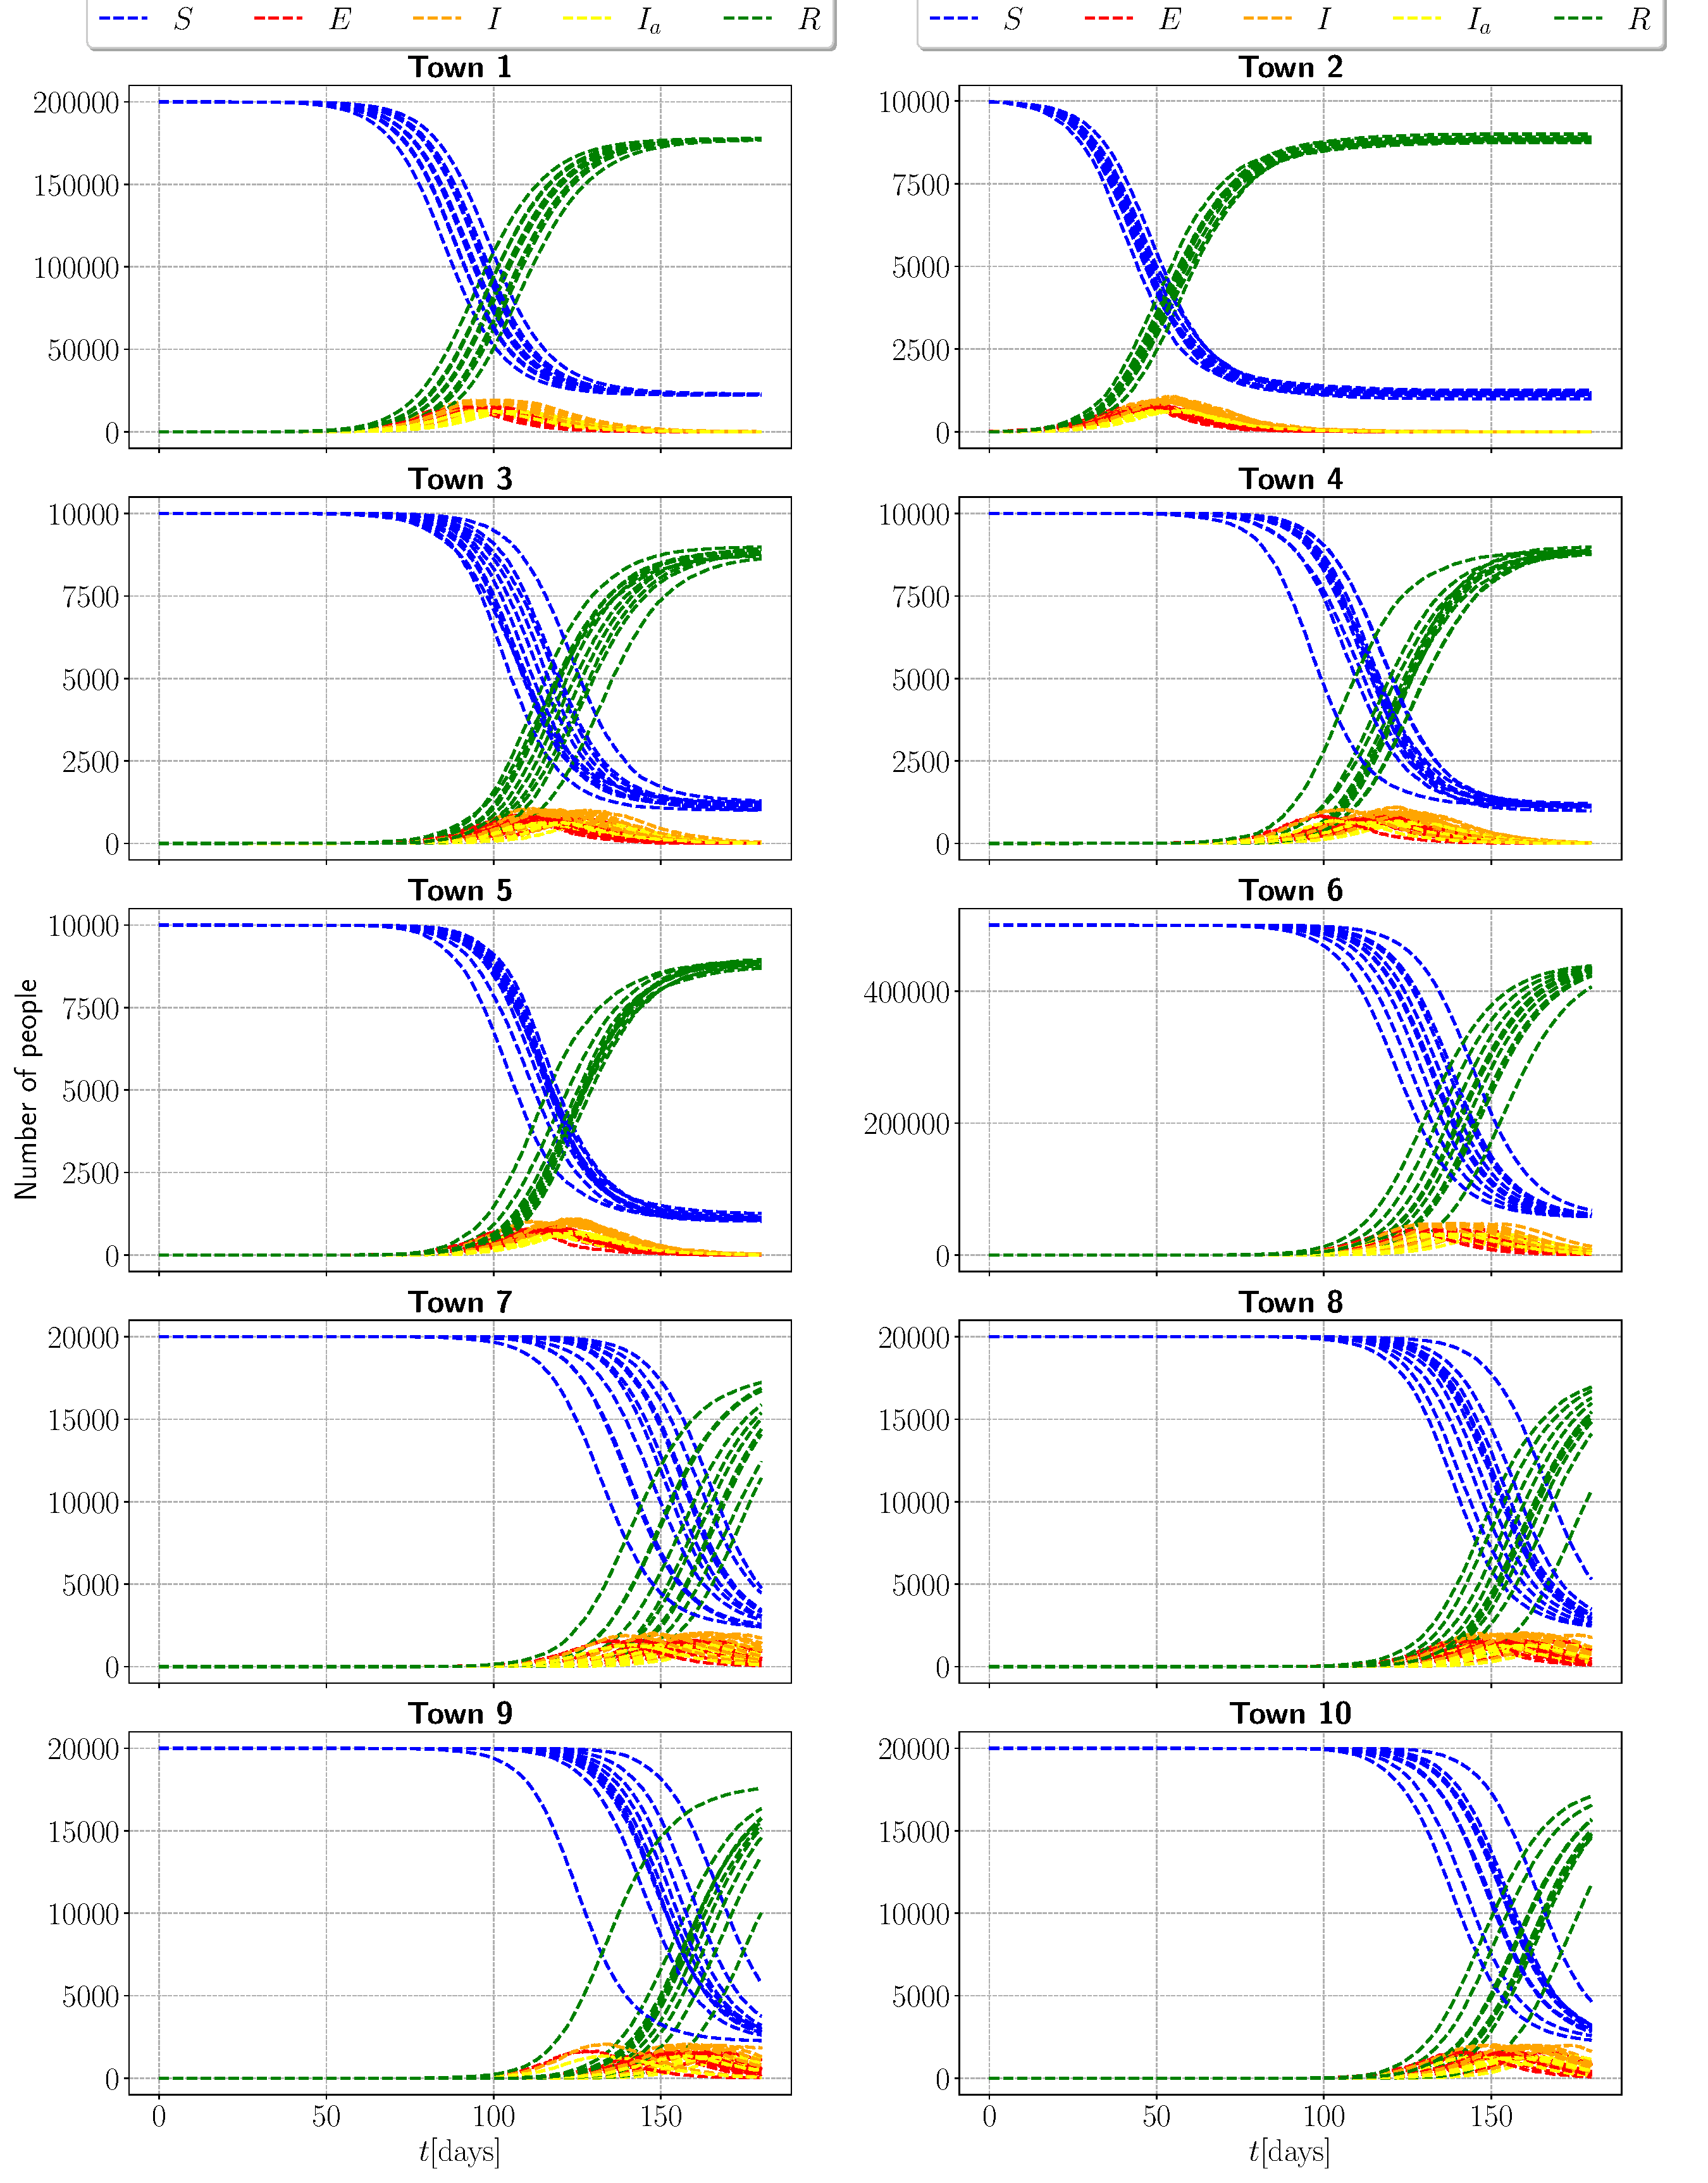
\includegraphics[width=0.9\columnwidth]{../fig/2Ea_commuter.pdf}
	\caption{Solutions of Stochastic SEIIaR commuter model for the $10$-city scenario.}
	\label{fig:commuter_10city}
\end{figure}

We use the framework developed in the previous section to simulate a larger system of towns, now with $10$ of them. The population matrix for this system is given in equation (11) in the problem sheet \cite{sheet}. We initialise the system with all people susceptible, except for $25$ exposed in town $2$. The time evolution of $10$ realisations of the different states is shown in figure \ref{fig:commuter_10city}. 

Figure \ref{fig:commuter_10city} clearly shows that the epidemic evolves fastest in town $2$, where it began. This is as expected. Furthermore, we see that the second fastest evolution is in town $1$, which is the closest connection to town $2$ in the sense that the commuters of town $2$ only travels to town $1$. This is also a reassuring fact, indicating a correct implementation. Interestingly, for the towns with more less connections to town $2$ --- e.g. town $9$ and $10$ --- we see that the evolution lags approximately $100$ days behind, and there seems to be a wider spread between each of the $10$ realisations. The increasing spread may be explained by the fact that small delays in each realisation in the beginning become exceedingly large for another town, as some time must naturally pass for the infections to be exported here.

\subsection{b) $356$ city simulation}

In this problem we use the full population structure as handed out along with the problem set. We are here only interested in the number of municipalities with more than $10$ infected people as a function of time ($\coloneqq \mathcal{N}(t)$), so we modify the commuter solver shown in listing \ref{lst:commuter} to only keep the current and previous state of the system at each time step, and calculate $\mathcal{N}$ for each time step. This is done to avoid using too much memory, which becomes a real problem if we try to allocate space for some thousand matrices of size $365 \times 365 \times 5$. 

$\mathcal{N}(t)$ for 10 realisations of this simulation is shown in figure \ref{fig:infected_Eb}.  

\begin{figure}[htb]
	\centering
	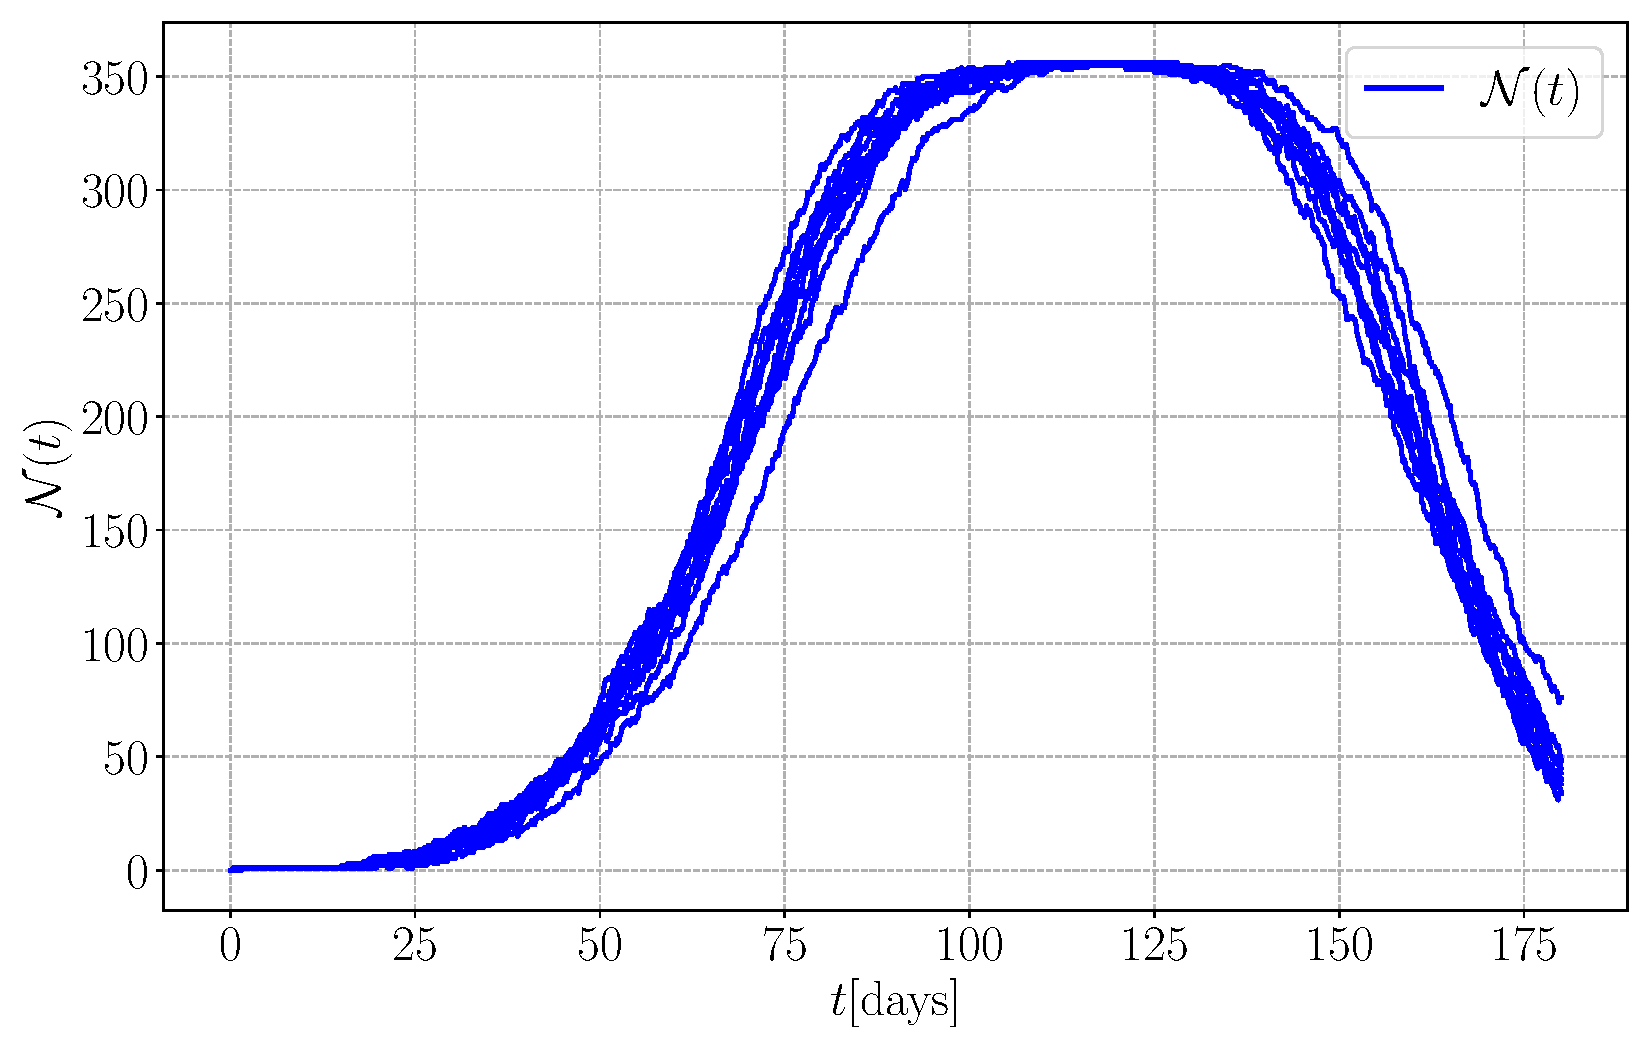
\includegraphics[width=0.9\columnwidth]{../fig/2Eb_N_back.pdf}
	\caption{Number of municipalities with more than $10$ infected people a a function of time.}
	\label{fig:infected_Eb}
\end{figure}
